% Created 2017-10-09 Mon 10:50
\documentclass[11pt]{article}
\usepackage[utf8]{inputenc}
\usepackage[T1]{fontenc}
\usepackage{fixltx2e}
\usepackage{graphicx}
\usepackage{longtable}
\usepackage{float}
\usepackage{wrapfig}
\usepackage{rotating}
\usepackage[normalem]{ulem}
\usepackage{amsmath}
\usepackage{textcomp}
\usepackage{marvosym}
\usepackage{wasysym}
\usepackage{amssymb}
\usepackage{hyperref}
\tolerance=1000
\usepackage[left=1in,right=1in,top=1in,bottom=1in]{geometry}
\usepackage{amsmath}
\date{October 9, 2017}
\title{Week 7 lecture notes - PSYC 5316}
\hypersetup{
  pdfkeywords={},
  pdfsubject={},
  pdfcreator={Emacs 25.2.1 (Org mode 8.2.10)}}
\begin{document}

\maketitle

\section*{Linear regression modeling}
\label{sec-1}

This week, we will talk about a classic technique in behavioral and social sciences: linear regression.  After discussing what it is and how to do it (at its most basic form), we will step back and develop TWO techniques for linear regression: one based on \emph{minimizing squared errors}, and another based on \emph{maximum likelihood estimation}.

\section*{Linear equations}
\label{sec-2}

Recall from algebra that any line can be written as $y=mx+b$, where $m$ is the slope and $b$ is the y-intercept.

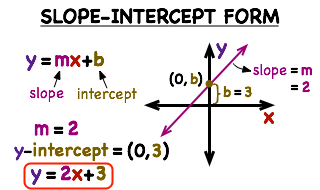
\includegraphics[width=.9\linewidth]{figures/week7/slopeIntercept.png}

In applied contexts, we usually write this equation as $y=a+bx$.  

\section*{What is a "linear model"?}
\label{sec-3}

To fit a "linear model" to data, we are making an assumption about the dependency between two variables.  Lets generate some data to see what I'm talking about:

\begin{verbatim}
N = 100
x = runif(N)
y = 3 + 5*x + rnorm(N)
plot(x, y, ylim=c(0,10))
\end{verbatim}

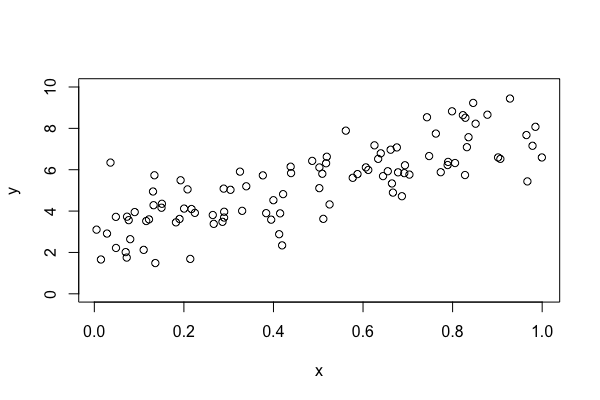
\includegraphics[width=.9\linewidth]{figures/week7/randomLinear.png}

It looks like $y$ varies linearly with $x$..that is, as $x$ increases, so does $y$, and the overall pattern looks like a straight line (with noise, of course).

So, we define the following model:

\[
y_i = a + bx_i + \varepsilon_i
\]

Note the index $i$ represents the different measurements in our sample $x_i$ and $y_i$ for $i=1,\dots, n$, and $\varepsilon_i$ represents the \textbf{measurement error} on the $i^{\text{th}}$ measurement.  These are sometimes called \textbf{residuals}.

Once we've defined the model, we need to find the \textbf{parameters} of the model: in other words, what are the values for intercept $a$ and slope $b$ that \emph{best fit} the data.  

Thus, "fitting a linear model" equates to a "parameter search", where we find the "best fitting" parameters for a given set of data.  To see this in action, we will play around with a simple demo here \url{https://www.geogebra.org/m/dlsxY1uX}

This demo starts with a set of 5 points and a line.  You can change the slope and intercept.  You can also see the residuals (and the squared residuals).  When playing around with this, you should think about what "best fit" would mean.  How do you find the "best fit"?  That is the subject for today's lecture.

\section*{Method 1: the "easy" way}
\label{sec-4}

This is an old problem, and as such, there are well-established methods for solving it.  We will begin by using the base function \texttt{lm} in R to find the parameters that fit the data.

\begin{verbatim}
model1 = lm(y~x)
summary(model1)
\end{verbatim}

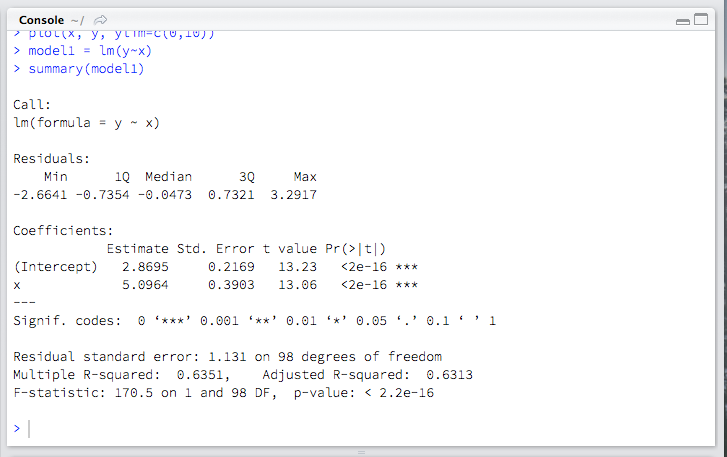
\includegraphics[width=.9\linewidth]{figures/week7/lmOutput.png}

The output is quite busy, but there are ways to extract vital information from the model.  First, let's plot the "best fitting line":

\begin{verbatim}
intercept = model1$coefficients[1]
slope = model1$coefficients[2]
abline(a=intercept, b=slope)
\end{verbatim}

The first two lines "extract" the intercept ($a$) and slope ($b$) from the \texttt{model1} object in R.  The third line (\texttt{abline}) plots the line on top of our data!

Beyond "fitting" the data quite well, we can use this model for another very important function: \textbf{prediction}.  For example, suppose we wanted to predict the value of $y$ for a given $x=0.5$.  Then we can just use the linear equation from our model to predict our value for $y$:

\begin{align*}
y & = a + bx\\
  & = 2.87 + 5.10x\\
  & = 2.87 + 5.10(0.5)\\
  & = 5.42\\
\end{align*}

Lets look at the errors/residuals. 

\begin{verbatim}
plot(density(model1$residuals))
\end{verbatim}

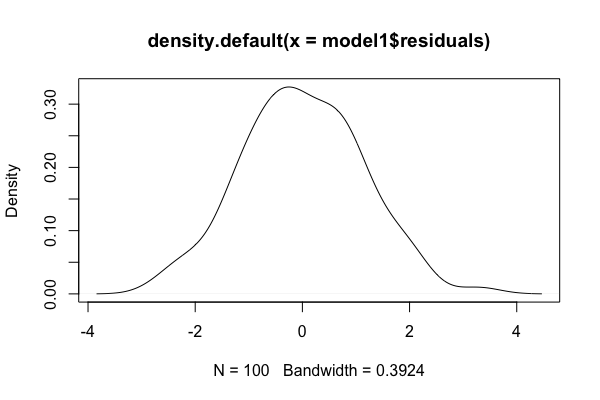
\includegraphics[width=.9\linewidth]{figures/week7/residuals.png}

Notice that the residuals seem to be normally distributed, centered at 0.  This is good, as it means that, on average, the error in our model is 0, and over-estimates are balanced with under-estimates.  This is generally regarded as a \emph{good fit}.

\subsection*{Example with real data}
\label{sec-4-1}

The following data represents some properties of various professions.  We will be interested in the relationship between education and income.

\begin{verbatim}
data = read.csv("https://git.io/vd2w3")
plot(data$education, data$income)
\end{verbatim}

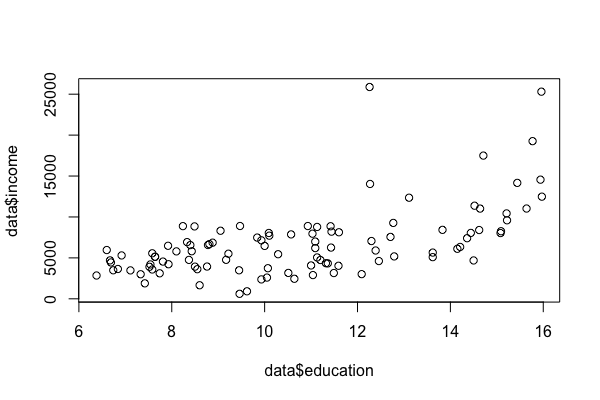
\includegraphics[width=.9\linewidth]{figures/week7/incomePlot.png}

Lets fit a linear model:

\begin{verbatim}
model2 = lm(data$income ~ data$education)
summary(model2)
intercept = model2$coefficients[1]
slope = model2$coefficients[2]
abline(a=intercept, b=slope)
\end{verbatim}

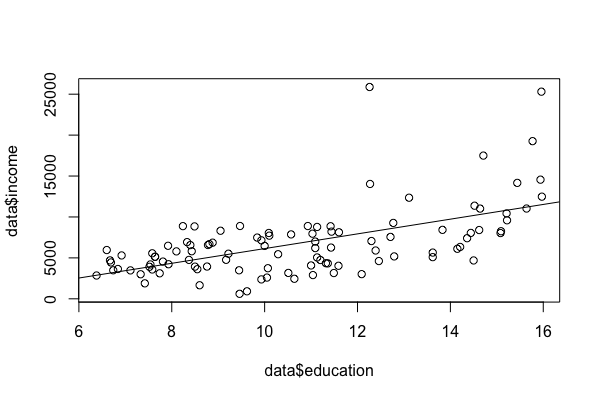
\includegraphics[width=.9\linewidth]{figures/week7/incomeFitted.png}

We can see that the line looks like a good fit, but lets look at the residuals.

\begin{verbatim}
plot(density(model2$residuals))
\end{verbatim}

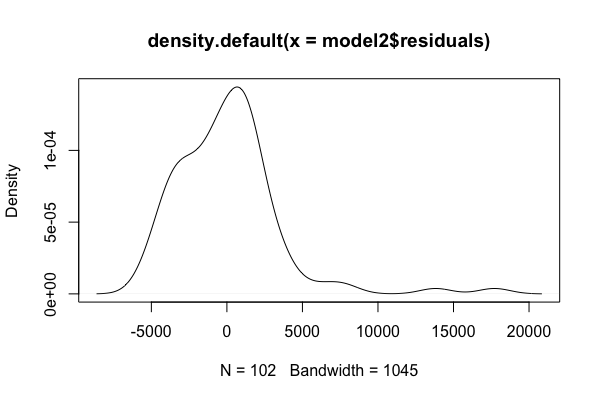
\includegraphics[width=.9\linewidth]{figures/week7/incomeResiduals.png}

The residuals peak at 0 (so most of our measurement error is 0), but we seem to have more underestimates (positive residuals) than overestimates (negative residuals).  Thus, this is not a \emph{great} fit, but OK.

\section*{Method 2 -- minimizing squared error}
\label{sec-5}

We will now talk about \textbf{how} to fit a linear regression model.  The first method we will discuss is the classical "OLS" method (ordinary least squares).  The basic idea is to compute errors between actual and predicted values, square them to get rid of negatives, and then find the parameters $a$ and $b$ which minimize this "squared error".

Mathematically, we want to find parameters $a$ and $b$ that minimize:

\[
\sum \varepsilon_i^2 = \sum (y_i - (a+bx_i))^2
\]

We can do this in R using the \texttt{optim} command.

First, we define a function that calculates the sum of squared errors:

\begin{verbatim}
SS = function(data,par){
  with(data, sum((y-(par[1]+par[2]*x))^2))
}
\end{verbatim}

As we did with maximum likelihood estimation in Week 2, this function takes two arguments: \texttt{data} and \texttt{par}.  In this context, \texttt{data} will be a data frame with two columns (\texttt{x} and \texttt{y}), and \texttt{par} will be a vector containing our parameters $a$ (\texttt{par[1]}) and $b$ (\texttt{par[2]}).

To find $a$ and $b$ that \textbf{minimize} this sum-of-squares function, we will use \texttt{optim} with a reasonable guess for initial values:

\begin{verbatim}
dat=data.frame(x,y)
inits=c(1,1)
optim(inits, SS, data=dat)
\end{verbatim}

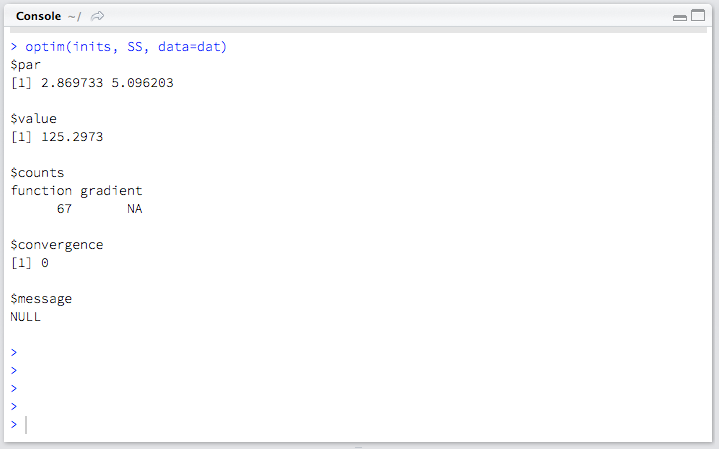
\includegraphics[width=.9\linewidth]{figures/week7/SS.png}

As you might expect, our fitted parameters $a$ and $b$ are the same as we got when we used the \texttt{lm} function earlier.

Lets try this with our other example (the education versus salary data):

\begin{verbatim}
dat=data.frame(data$education, data$income)
names(dat) = c("x", "y")
inits=c(1,1)
optim(inits, SS, data=dat)
\end{verbatim}

As you will see, the parameter estimates for $a$ and $b$ are almost exactly the same as we obtained with the \texttt{lm} command.

\section*{Method 3 -- maximum likelihood estimation}
\label{sec-6}

Instead of minimizing the sum of squared errors, we can use maximum likelihood estimation.  This requires a bit more sophistication in our definition of a \textbf{linear model}.  So, lets start there.

Recall that for MLE, one needs a likelihood function.  That is, we need some sort of distributional assumption to proceed (e.g., is something normally distributed)?  Recall that in a linear model, we have

\[
y_i = a+bx_i + \varepsilon_i
\]

or rewritten

\[
\varepsilon_i = y_i - (a+bx_i)
\]

We want the residuals $\varepsilon_i$ to be centered at 0.  Thus, one way to do this is to place a \textbf{normal} model on the residuals.  That is, we assume

\[
\varepsilon_i \sim \text{Normal}(0, \sigma^2)
\]

So, this is a problem that MLE can solve!  We simply need to find parameters $a$ and $b$ so that $y_i-(a+bx_i)$ is normally distributed with mean 0 and variance $\sigma^2$.

As in week 2, we begin by defining a negative log-likelihood (NLL) function:

\begin{verbatim}
reg.nll = function(data, par){
  residual = with(data, y-(par[1]+par[2]*x))
  return(sum(-log(dnorm(residual, mean=0, sd=par[3]))))
}
\end{verbatim}

Then, we minimize this NLL via the \texttt{optim} function.

\begin{verbatim}
dat=data.frame(x,y)
inits=c(3,5,2)
optim(inits, reg.nll, data=dat)
\end{verbatim}

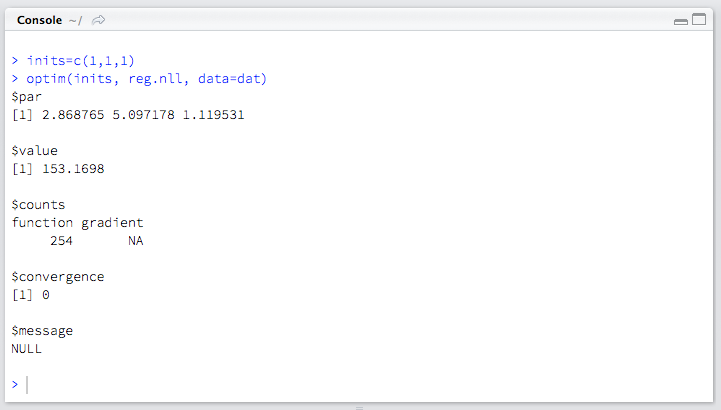
\includegraphics[width=.9\linewidth]{figures/week7/mle.png}

Notice that we get the same estimates for $a$ and $b$ as before.  This time, we also get an estimate for $\sigma$, the standard deviation of the residual distribution.

\subsection*{Confidence intervals on parameter estimates}
\label{sec-6-1}

One of the advantages to the MLE approach is that we can easily compute confidence intervals for our estimates.  
% Emacs 25.2.1 (Org mode 8.2.10)
\end{document}